\chapter{Introduction}
\label{chap:theory}

\section{The Standard Model of Particle Physics}
\label{sec:theSM}

The \ac{SM} of fundamental interactions is the theory
which describes the electromagnetic, weak and strong nuclear interactions, often
represented as a collection of the elementary particles predicted by the theory.
The SM has successfully described data from a wide range of experiments, and in the 
years prior to the LHC, all of the predicted elementary particles were verified 
except for one: the Higgs boson.

\subsection{Particles and Forces} 

The \ac{SM} is a renormalisable quantum field theory, in which the constituents of
matter are represented as spin-$\frac{1}{2}$ fermions which interact with
forces mediated by spin-1 bosons. These interactions are described by a
Lagrangian which is invariant under $SU(3)_{C} \times SU(2)_{L} \times U(1)_{Y}$
symmetries. The $SU(3)_{C}$ part describes the strong interaction, mediated by
particles which carry colour charge (C). In these interactions, described by the
theory of \ac{QCD}\cite{}, the force mediators are massless gluons
and the coloured fermions are the quarks. The remaining fundamental fermions,
the leptons, do not carry colour charge and hence do not interact via the strong
force. Both the leptons and quarks participate in electroweak interactions,
which are governed by the $SU(2)_{L} \times U(1)_{Y}$ symmetry.

The electroweak symmetry describes the unified electromagnetic and weak
interactions\cite{}, and was one of the major achievements of the twentieth
century in the \ac{SM}. In electroweak theory the quantum numbers of interest are
weak isospin $t_{1,2,3}$ and hypercharge $y$. These are related to the
electric charge Q as: 

\begin{equation}
Q = t_{3} + \frac{y}{2}
\end{equation}

The gauge fields associated with these quantum numbers are the three weak isospin fields,
$W_{\mu}^{i}$, $i = 1,2,3$, and the hypercharge field $B_{\mu}$. The weak
isospin fields act on doublets: 

\begin{equation}
\begin{pmatrix} u_{i} \\ d_{i} \end{pmatrix}_{L} ,   
\begin{pmatrix} \nu_{i} \\ {l_{i}} \end{pmatrix}_{L}
\end{equation}

where $u_{i}$ are the up-type quarks ($u,c,t$), $d_{i}$ are the down-type quarks
($d,s,b$), $l_{i}$ are the charged leptons ($e,\mu,\tau$) and $\nu_{i}$ are the
corresponding neutrinos ($\nu_{e},\nu_{\mu},\nu_{\tau}$). The index $i$ indicates first, second or third
generation fermions. The subscript $L$ indicates that the doublets correspond to
the left handed projection of the fermions. The weak force only interacts with
left handed fermions, and as such is maximally parity violating. The right handed projections
transform as singlet states, which are invariant under $SU(2)_{L}$.

The physical $\gamma, Z$ and $W$ bosons result from mixing between the gauge
fields:

\begin{equation}
\begin{pmatrix} A_{\mu} \\ Z_{\mu}^{0} \end{pmatrix} = 
\begin{pmatrix} \cos{\theta_{W}} & \sin{\theta_{W}} \\ -\sin{\theta_{W}} &
\cos{\theta_{W}} \end{pmatrix} . 
\begin{pmatrix} B_{\mu} \\ W_{\mu}^{3} \end{pmatrix}
\end{equation}

where $A_{mu}$ is the photon field and $\theta_{W}$ is the weak mixing angle,
which can be related to the couplings of the weak neutral ($g$) and electromagnetic
interactions ($g'$) as $\theta_{W}=\tan^{-1}{\frac{g'}{g}}$. 

No mass terms. Need to add either lagrangian to prove this or find a hand wavey
way using the doublets and the interaction terms. Then we move on to EWSB,
having motivated it.

\cite{GlashowPartialSymmetries,WeinbergModelOfLeptons,SalamNobelSymposium}.

\subsection{The Higgs Mechanism in the \ac{SM}}
\label{sec:SMHiggs}


\begin{figure}[htbp]
   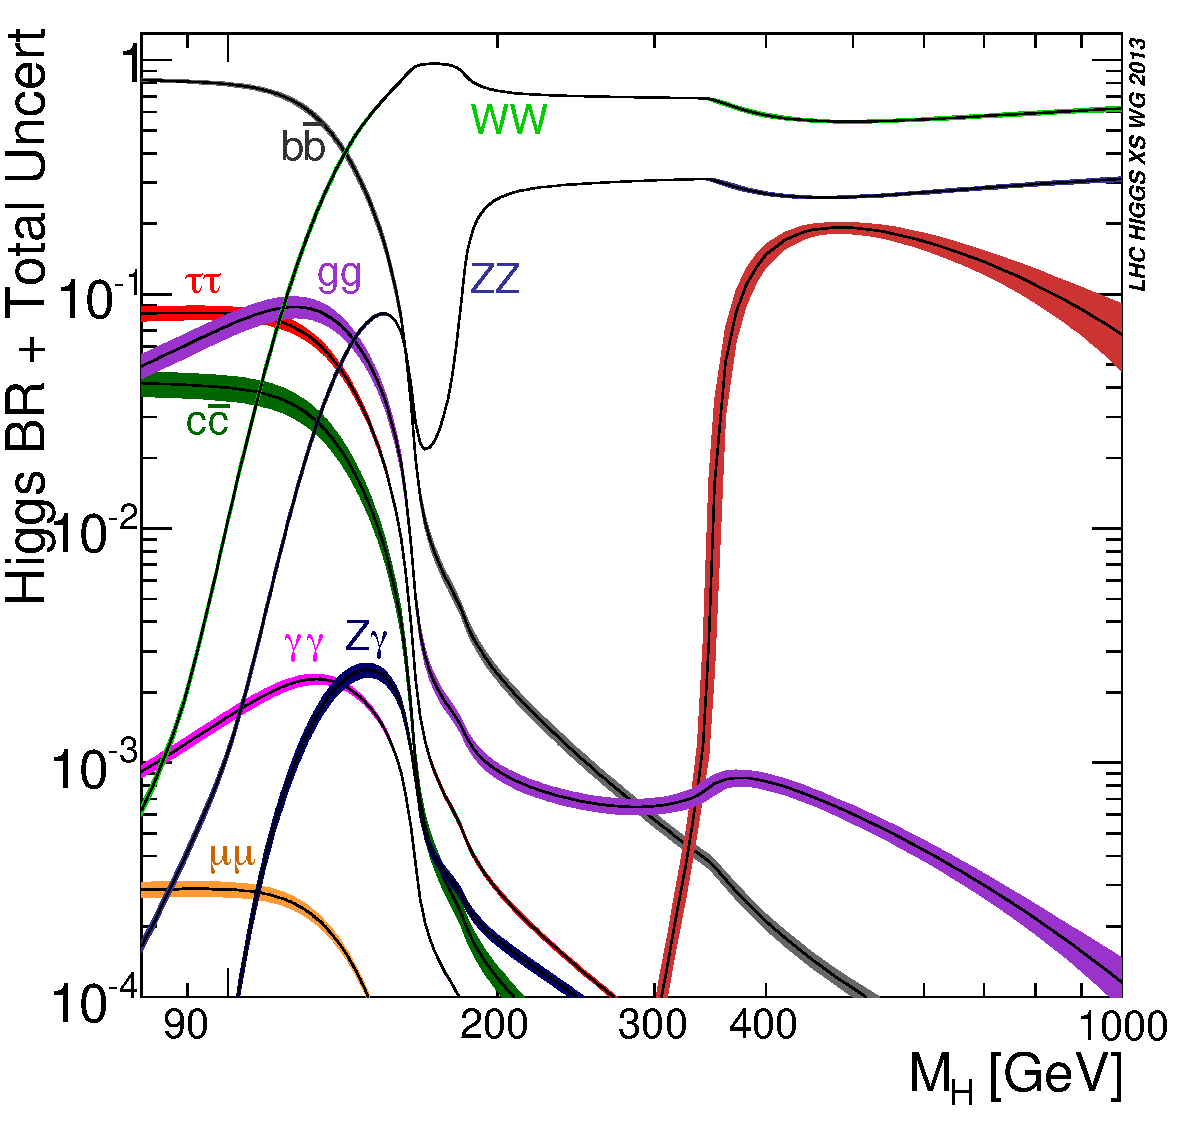
\includegraphics[width=0.5\textwidth]{plots/theory/Higgs_BR.pdf}
\caption{Higgs boson branching ratios in the \ac{SM}\cite{}.}
\label{fig:SMHiggsBRs}
\end{figure}


\subsection{Motivation for theories beyond the \ac{SM}}

Despite its successes, the \ac{SM} is known to have some shortcomings. One concerns
the calculations of the Higgs Boson mass, and is known as the Hierarchy problem. 

\section{Theories beyond the SM}
\label{sec:BSM}

\subsection{The Higgs sector in the MSSM}
\label{sec:mssmhiggs}

\subsection{MSSM Models incorporating the LHC Higgs}
\label{sec:mssmbenchmarks}

\section{Previous Searches}




